\section{Running the simulation}

\paragraph{}
Other users of this code may choose to make adjustments to better suit their needs, but for now, this is how the code is generally run. Not every command will be reviewed here, but a general description of the procedure will be provided. 

\begin{figure}[h]
    \begin{center}
    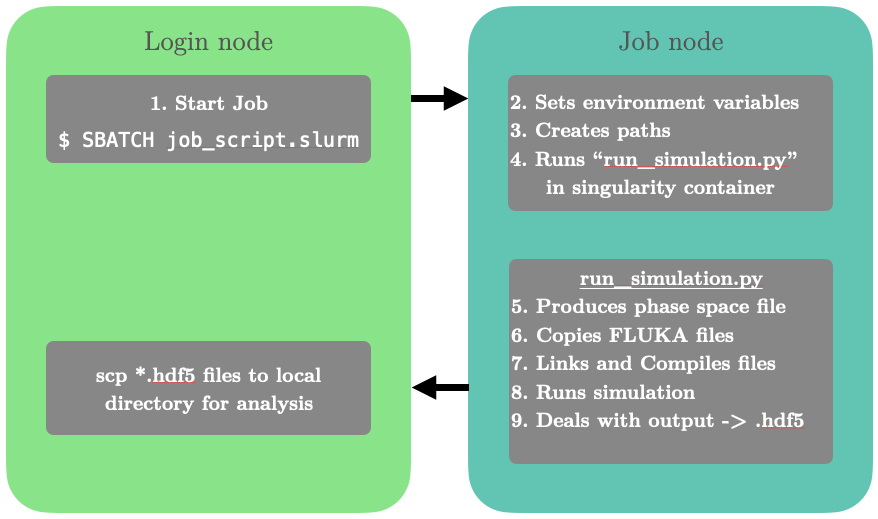
\includegraphics[scale=0.5]{figures/nodes.png}
    \caption{A simple display of what is happening when the code is run}
    \label{fig:running}
    \end{center}
\end{figure}

\paragraph{Preparing Inputs}
First, the user must be sure of how many muons ought to be simulated and what size the targetting region should be. The yaml file should be configured to match these specifications. Apt file names should be assigned for outputs. These can be changed from within the SLURM file. 

\paragraph{Running}
The only remaining step in running the simulation is to execute the SLURM file; this requests the necessary resources to run a batch of simulations simultaneously and moves the output to the specified paths: \begin{verbatim}
    $ sbatch job_script.slurm
\end{verbatim}


\paragraph{Analyzing the HDF5 files}
Now the user is free to analyze the resultant hdf5 files which contain the necessary FLUKA outputs.